\documentclass[]{scrartcl}
\usepackage{lmodern}
\usepackage{amssymb,amsmath}
\usepackage{ifxetex,ifluatex}
\usepackage{fixltx2e} % provides \textsubscript
\ifnum 0\ifxetex 1\fi\ifluatex 1\fi=0 % if pdftex
  \usepackage[T1]{fontenc}
  \usepackage[utf8]{inputenc}
\else % if luatex or xelatex
  \ifxetex
    \usepackage{mathspec}
  \else
    \usepackage{fontspec}
  \fi
  \defaultfontfeatures{Ligatures=TeX,Scale=MatchLowercase}
\fi
% use upquote if available, for straight quotes in verbatim environments
\IfFileExists{upquote.sty}{\usepackage{upquote}}{}
% use microtype if available
\IfFileExists{microtype.sty}{%
\usepackage[]{microtype}
\UseMicrotypeSet[protrusion]{basicmath} % disable protrusion for tt fonts
}{}
\PassOptionsToPackage{hyphens}{url} % url is loaded by hyperref
\usepackage[unicode=true]{hyperref}
\hypersetup{
            pdftitle={Introductory Essay},
            pdfborder={0 0 0},
            breaklinks=true}
\urlstyle{same}  % don't use monospace font for urls
\IfFileExists{parskip.sty}{%
\usepackage{parskip}
}{% else
\setlength{\parindent}{5pt}
\setlength{\parskip}{10pt plus 4pt minus 1pt}
}
\setlength{\emergencystretch}{3em}  % prevent overfull lines
\providecommand{\tightlist}{%
  \setlength{\itemsep}{0pt}\setlength{\parskip}{1pt}}
\setcounter{secnumdepth}{0}
% Redefines (sub)paragraphs to behave more like sections
\ifx\paragraph\undefined\else
\let\oldparagraph\paragraph
\renewcommand{\paragraph}[1]{\oldparagraph{#1}\mbox{}}
\fi
\ifx\subparagraph\undefined\else
\let\oldsubparagraph\subparagraph
\renewcommand{\subparagraph}[1]{\oldsubparagraph{#1}\mbox{}}
\fi

% set default figure placement to htbp
\makeatletter
\def\fps@figure{htbp}
\makeatother

%custom options
\usepackage{lineno}
\usepackage{multicol}
\setmainfont{Source Serif Pro}
\setsansfont{IBM Plex Sans}
\usepackage{graphicx}

%options for images
\renewcommand\floatpagefraction{.95} % for two column documents
\renewcommand\topfraction{.95} % for two column documents
\renewcommand\bottomfraction{.9}
\renewcommand\textfraction{.1}
\setcounter{totalnumber}{50}
\setcounter{topnumber}{50}
\setcounter{bottomnumber}{10}
\setlength{\textfloatsep}{10pt}
\setlength{\floatsep}{10pt}
%

\title{Introductory Essay}
\author{Pratik R Gupte}
\date{January 2019}

\begin{document}
\maketitle

\newpage

\textbf{© Pratik R Gupte}

\textbf{Modelling Adaptive Response Mechanisms Group},

Groningen Institute for Evolutionary Life Sciences,

University of Groningen

\textbf{Bijleveld Lab},

Department of Coastal Systems,

Royal Netherlands Institute for Sea Research

\textbf{Contact information}

Groningen Institute for Evolutionary Life Sciences\\
University of Groningen\\
Nijenborgh 7-5172.0583, 9747 AG Groningen \\
Netherlands\\
p.r.gupte@rug.nl

\textbf{Supervisors}

FJ Weissing\\
AI Bijleveld\\
AGG Groothuis\\
T Piersma

\textbf{Promotors}

FJ Weissing\\
AGG Groothuis

\textbf{Funding}

Adaptive Life Programme -- Groningen Institute for Evolutionary Life
Sciences\\
Short term causes and long term consequences of adaptations to
environmental change

\newpage

\tableofcontents

\newpage \mbox{} \pagebreak

\part{Summary}\label{summary}

The \emph{\textbf{movement of animals}} has always fascinated humans,
but modern biology has only now come to actively study movement as the
linchpin of many processes. As movement studies seek to unify phenomena
across scales, they must also contend with the idea that there are
\emph{\textbf{consistent individual differences}} within many animal
populations. These differences, whose evolution, development, and
maintenance are still under debate, are estimated to have population
level consequences. One system in which consistent individual
differences have been identified is that of \emph{\textbf{red knots}}
\emph{Calidris canutus}, which forage on intertidal mudflats and vary
along an axis of exploratory behaviour. Knots' and other foragers'
movement is often strongly influenced by which
\emph{\textbf{spatio-temporal change}} in the often unpredictable
resource landscape. This system inspires questions about how movement
strategies evolve in such landscapes, how they affect the landscapes on
which they evolve, as well as how the interaction of the two gives rise
to emergent phenomena such as structured communities. Those questions
will be the subject of my thesis.

This essay, an introduction to my work over the next two years, is
organised in the following sections: first, the
\emph{\textbf{Introduction}} contains key concepts in the fields of
\emph{Animal movement, Movement as personality,} and \emph{Modelling
movement}. The second section, \emph{\textbf{About this project}}, lays
out the questions I want to investigate. The third section,
\emph{\textbf{Towards a model of wader movement}}, explains the
conceptual and practical aspects of the models and empirical methods I
propose to implement towards goals in Section 2.

\begin{linenumbers}
	
\part{Introduction}\label{introduction}
    \section{Animal movement}\label{animal-movement}

Animal movement across spatio-temporal scales -- from seasonal
migration, to breeding aggregations, to diurnal cycles -- have been an
important field of human knowledge throughout recorded history, and
likely long before. Even in more modern times, the two most successful
paradigms of the natural sciences' century of insight, evolution by
natural selection (Darwin and Wallace 1858) and island biogeography
(MacArthur and Wilson 2001), rely at least in part on the movement of
animals to make their point. Explicit treatment of the subject began
with theoretical developments on the movement of freely moving and
ideally rational agents. This led to nearly simultaneous advances in the
understanding of the distribution of foragers at the landscape scale
(Fretwell and Lucas 1970), and the topology of groups of selfish agents
(Hamilton 1971). Theory on population spatial distributions soon
incorporated fine-scale phenomena such as individual interactions and
population structure, and was already a mature field with strong
empirical support when reviewed by Sutherland 1996. Theoretical advances
in the study of fine-scale movement itself, on the other hand, have
lagged behind the measurement of the movement of individual animals
(Holyoak et al. 2008).

The recently emerged movement ecology paradigm (MEP; Nathan et al. 2008)
has sought to fill this gap, understanding ``movement itself as the
focal theme\ldots{}by providing a unifying framework and common tools''
(Nathan 2008). This paradigm urges practitioners to attempt to answer
three questions: 1. \emph{Why} do organisms move? 2. \emph{Where} do
organisms decide to move? 3. \emph{How} do organisms move? This links
(1) external stimuli, such as fear of predators (Laundre et al. 2001),
(2) sensory capacity, which translates into navigational ability and
search strategies (eg. Bartumeus and Levin 2008), and (3) life-history
dependent physiology and internal state (eg. Fryxell et al. 2008).
Movement ecology's rise has coincided with the beginning of ``a golden
age of animal tracking science'' in the form of large-scale and
high-resolution animal tracking (Hussey et al. 2015, Kays et al. 2015).
Biologging, i.e., the remote measurement of instantaneous organism state
(Cooke et al. 2004), and high-resolution animal tracking in particular,
have led to remarkable insights into the detailed sub-units of movement
behaviour, such as the energetics of predation and locomotion (see eg.
Williams et al. 2004, Scantlebury et al. 2014).

\begin{figure}
	\centering
	\includegraphics[width=0.7\linewidth]{fig02_nathan_etal_2008}
	\caption{The movement ecology paradigm places observed movement (\textit{path: U}) as both a consequence of prior factors, and a contributor to future ones. From Nathan et al. (2008).}
	\label{fig:fig02nathanetal2008}
\end{figure}

Despite advances in empirical methods, animal movement studies are still
subject to limitations of scale. Among these are emergent group-size
effects (Tunstrøm et al. 2013), which are difficult to quantify empirically
notwithstanding recent advances (Handegard et al. 2012, Kays et al.
2015, Strandburg-Peshkin et al. 2015, Dhanjal-Adams et al. 2018); a
distinct problem when animal grouping is near-universal (Krause and
Ruxton 2002). The impracticality of research across scales of
organisation (eg. physiology to population) has similarly confined most
movement studies to answering at most one MEP question at a time (but
see Fryxell et al. 2008, Strandburg-Peshkin et al. 2015, Curtin et al.
2018). This is linked to the choice of study system, which among
vertebrates has been restricted by the technical difficulty in hewing to
the 3\% body-mass rule (Naef-Daenzer et al. 2001). Finally, animal
movement has been captured by the movement \emph{ecology} paradigm
because of the difficulty in studying movement at evolutionary
timescales. Here, simulation models can help to shine ``the light of
ecology'' on evolutionary biology (Grant and Grant 2011), by uncovering
the importance of individual interactions for emergent phenomena (eg. Hildenbrandt
et al. 2010, Tunstrøm et al. 2013), the surprising extrinsic drivers of
movement mode (Guttal et al. 2012), the evolutionary effects of higher
trophic levels (Ioannou et al. 2012), and the evolution of movement
rules (de Jager et al. 2011, Netz 2017).



\section{Movement as personality}\label{movement-as-personality}

The work cited above may be safely claimed to make at least one of two
assumptions; the first is that of the `golden mean'. The second is the assumption of
optimality (Fretwell and Lucas 1970) entailing infinite behavioural
plasticity. Neither of these assumptions is very well founded. While the
first is methodologically convenient, theory from Darwin 1859 onwards
has recognised it as untrue; models find that differences among
individuals can have population level consequences (eg. Pruitt and
Riechert 2011). The second assumption is squarely challenged by the
study of consistent individual differences in behaviour. The field of
animal personality and behavioural syndromes (Sih et al. 2004a, b) and
its consequences
(\protect\hypertarget{__UnoMark__44474_2549695377}{}{\protect\hypertarget{__UnoMark__53900_4107183634}{}{\protect\hypertarget{ZOTERO_BREF_pK0LuydZRLN9}{}{\protect\hypertarget{__UnoMark__39595_623588325}{}{}}}}Dingemanse
and Réale 2005) seeks to quantify between and within individual
consistency in behavioural responses ``through time or across
situations''. Variation along two or more axes of personality
(\protect\hypertarget{__UnoMark__44475_2549695377}{}{\protect\hypertarget{ZOTERO_BREF_S1piFXmJVFzL}{}{\protect\hypertarget{__UnoMark__53901_4107183634}{}{\protect\hypertarget{__UnoMark__39596_623588325}{}{}}}}Réale
et al. 2007) may be correlated into a `behavioural type' (examples in
Sih and Bell 2008, Bell et al. 2009); for example, `boldness' and
`aggression' form two of the major axes of personality, and are often
quantified together as a syndrome (Carter et al. 2013).

Behavioural ecology has only slowly come to terms with the idea that
such individual differences within populations could be advantageous
(Wilson 1998). Individual differences have been explained in terms of
mechanisms engaged during development (Wolf and Weissing 2010, Groothuis
and Trillmich 2011), trade-offs in life-history (Wolf et al. 2007a, b),
and the feedback loops created between individual state and behaviour
(Wolf and Weissing 2010) as prominent proximate causes. Evolutionary
explanations of these differences and especially their consistency have
remained elusive because the default expectation has been that
plasticity is more adaptive (Wilson 1998). Wolf and Weissing 2010 have
since shown that consistent behavioural types may yet achieve comparable
fitness outcomes if selection is frequency-dependent (Maynard Smith
1982), and rarer types have a selective advantage. Spatio-temporal
variation, a ubiquitous feature of environments (Levin 1992), may have a
major role to play when it hosts a population where infinite
adaptability is costly or habitat choice limited (Wolf and Weissing
2010). In such cases, individuals may specialise for particular spatial
or temporal conditions, maintaining global variability, while local
variability may be maintained through imperfect estimation of current
habitat state (Wolf and Weissing 2010, 2012). However, there is little
doubt that behavioural types have signficant eco-evolutionary
consequences for populations (Sih et al. 2012, Wolf and Weissing 2012).

The movement ecology paradigm places animal movement at the end of a
pipeline fed into by physiology, stimuli, and cognition (\emph{state},
Wolf and Weissing 2010, 2012), and it is unsurprising that populations
might have evolved behavioural polymorphisms for movement, or
\emph{movement types} (Wolf and Weissing 2010, Getz et al. 2015, Netz
2017). Indeed, movement types are inherent predictions of previous
theoretical work that did not necessarily consider movement as its
central theme (eg. Watson and Miller 1971, Lima and Zollner 1996).
Animal tracking has since confirmed such individual consistency in
movement across scales, from local movements (Austin et al. 2004,
Leclerc et al. 2016) to dispersal (Duckworth and Badyaev 2007, Clobert
et al. 2009, Cote J. et al. 2010, Duckworth and Sockman 2012). While
Wolf and Weissing 2010 suggested that some spatio-temporal environmental
variability might be causal to consistency evolution, later work showed
that such structure can be created from uniformity by individuals
themselves, and thus may be co-incidental rather than causal in relation
to movement strategy evolution (de Jager et al. 2011, Getz et al. 2015,
Netz 2017). In general, this points to the interplay between
individuals' movement and the landscapes -- and begs the question of how
rate and predictability of landscape change (\emph{sensu lato} Botero et
al. 2015) might affect the evolution of movement types. Spiegel et al.
2017 have demonstrated that this link betweenz movement types
(\emph{fast} and \emph{slow}; see parallels with earlier Wolf et al.
2007a, b) and fitness outcomes in landscapes that vary in spatial
\emph{predictability} can have consequences at the population level --
from social networks to community composition.

\begin{figure}
	\centering
	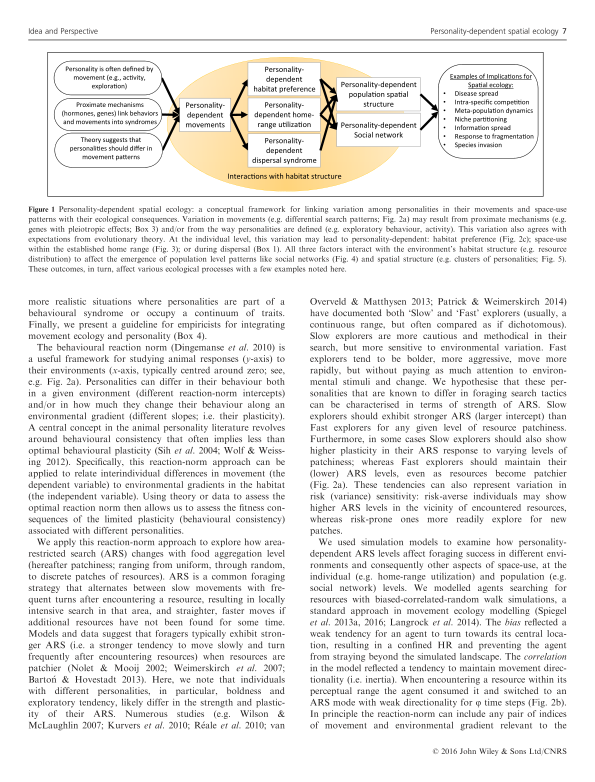
\includegraphics[width=0.7\linewidth]{fig01_spiegel_etal_2017}
	\caption{Spiegel et al. (2017) lay out a framework linking personality, movement, and resulting interactions. Personality may be initially measured in terms of movement, but the underlying causes can impact larger-scale processes such population spatial structure.}
	\label{fig:fig01spiegeletal2017}
\end{figure}


\section{Modelling movement}\label{modelling-movement}

Many aspects of personality and movement -- across scales -- can be
explored using the waders \emph{Charadrii,} and especially the
sandpipers Scolopacidae as a model system. Waders are a ubiquitous group
of long-lived birds characterised by their littoral foraging on buried
macrozoobenthic prey, and their often extreme flyway-channelled
migration between generally disjointed and strongly seasonal global
distributions (Boere and Stroud 2006, Gill et al. 2009, Piersma and
Bonan 2019). Sandpipers are well known for their huge wintering
fission-fusion flocks (Myers 1983, Conklin and Colwell 2008), and as
symbols of traditional landscapes (Colwell 2018). Waders (hereafter
referring to scolopacids) eking out their precarious existence
(Fitzpatrick and Senner 2018) at the waterline are thus poised to be the
new canary in the coalmine: harbingers of global environmental change
(\protect\hypertarget{__UnoMark__44501_2549695377}{}{\protect\hypertarget{ZOTERO_BREF_Jo6zuDEr7hJE}{}{\protect\hypertarget{__UnoMark__39624_623588325}{}{\protect\hypertarget{__UnoMark__53929_4107183634}{}{}}}}Piersma
and Lindström 2004, Wikelski and Tertitski 2016) which has swiftly
advanced from `near' to `here' (IPCC 2018). Wader movement fulfils many
of the requirements one would expect from a system that integrates
animal personality and movement studies. First, wader movement has been
extensively investigated using a variety of approaches at nearly all
spatio-temporal scales: small spatio-temporal scales such as foraging
(van Gils et al. 2003, van Gils 2010), large spatio-temporal scales such
as migration (Buehler et al. 2006, Piersma 2011), proximate causes for
large-scale phenomena (Lank et al. 2003, Ydenberg et al. 2004, Ruthrauff
et al. 2013, 2018), and ultimate causes for small-scale phenomena (van
Gils et al. 2006, Kraan et al. 2009a). Of the waders, red knots
\emph{Calidris canutus} are among the best studied, with a wealth of
biological information, from an understanding of physiology and its
interaction with exploratory personality (Bijleveld et al. 2014, Mathot
et al. 2017), to knowledge of group dynamics across scales (Bijleveld et
al. 2010, 2012b, 2015b), to the effect of foragers on their resource
landscapes (Bijleveld et al. 2015a).

Many theoretical studies increasingly employ agent-based approaches,
which were developed to overcome two flaws in mathematical models
(Huston et al. 1988). First, in order to prevent an unreasonably large
number of parameters (a disadvantage of ABMs), earlier models had
abstracted populations to ``golden mean'' values that elided individual
differences (see previous section) essential to evolutionary and
ecological processes. The second issue was the assumption of global
interactions, i.e., that all individuals affect all others equally,
ignoring central problems of scale (Levin 1992) and local interactions
(see Legendre 1993) in ecology. ABMs have since been standardised in
terminology (Grimm et al. 2006, 2010), and are widespread in ecology
(DeAngelis 2018). In such models, individual organisms are each modelled
separately and allowed to make decisions based upon various inputs, akin
to real decision making processes. In animal ecology, ABMs are
especially relevant in modelling movement (reviewed in DeAngelis and
Mooij 2005), and have been used extensively to model avian movement
including that of red knots (van Gils 2010, Spiegel et al. 2013, 2017,
Getz et al. 2015, 2016 etc). Simple evolutionary algorithms (see
\protect\hypertarget{ZOTERO_BREF_6WhVYsaNgj9a}{}{\protect\hypertarget{__UnoMark__44517_2549695377}{}{\protect\hypertarget{__UnoMark__39640_623588325}{}{\protect\hypertarget{__UnoMark__53945_4107183634}{}{}}}}Bäck
1996) as implemented in Getz et al. 2015, Netz 2017 that predicate the
reproductive output (replicates) of each agent on some measure of
fitness, such as net intake, can add evolutionary dynamics to otherwise
simple ABMs. This allows the modelling of movement across scales, from
small-scale within-patch dynamics, such as competition (Keddy 2001) and
the investigation of emergent large-scale evolutionary dynamics, such as
community composition (\emph{movement guilds}, Getz et al. 2015), and
alternative strategies (Netz 2017). A major advance may be made by
having the decisions of agents be the output of a `black-box' process in
the form of artificial neural networks (ANNs; Enquist and Ghirlanda
2013; see Netz 2017). Neural network approaches allow for surprising
results -- such as the evolution of rich movement dynamics and
alternative strategies, even when beginning from largely similar
populations (Netz 2017).

\newpage

\part{About this project}\label{about-this-project}

In this section, I outline my approaches to examine the
\emph{\textbf{evolution of movement types}} (sensu Wolf and Weissing
2010, Getz et al. 2015) in the context of \emph{\textbf{environmental
predictability and rate of change}} (as in Botero et al. 2015), using
the \emph{\textbf{red knot system}} as a reference
(\protect\hypertarget{__UnoMark__3976_580056431}{}{}Bijleveld et al.
2012b, 2014, 2015a, b, Oudman et al. 2018).
\protect\hypertarget{__UnoMark__3983_580056431}{}{}Wolf and Weissing
2010 lay out the theoretical basis for the expectation that consistent
behavioural differences arise in spatially structured landscapes, while
\protect\hypertarget{__UnoMark__3990_580056431}{}{}Botero et al. 2015
describe how environments in certain regimes of temporal variability and
predictability can give rise to similar polymorphisms.
\protect\hypertarget{__UnoMark__3997_580056431}{}{}Getz et al. 2015 and
\protect\hypertarget{__UnoMark__4004_580056431}{}{}Netz 2017 show how
virtual agents can evolve movement types while structuring initially
featureless landscapes. Bijleveld and colleagues (above) provide
empirical data on the foraging and movement ecology of red knots that
can inform modeling approaches and which may be used to test model
predictions.

\section{Abstract models}\label{abstract-models}

I will begin with an abstract approach and some basic questions.
Modelling agent movement as the output of an ANN which takes
environmental cues as outputs, I will first investigate how different
regimes of landscape patchiness and temporal variability influence the
evolution of movement types. Specifically, I will be interested in the
following:

\begin{enumerate}
\def\labelenumi{\arabic{enumi}.}
\item
  
  \emph{\textbf{How many movement types are evolved under different
  regimes of spatial predictability and variability?}} This question is
  aimed at unifying the Wolf and Weissing (2010) and Botero et al.
  (2015) approaches at broad evolutionary scales. Recent mechanistic
  models based on ANNs suggest that genotype-phenotype mapping is not as
  clear-cut as in Botero and colleagues' work, and that polymorphisms
  (there identified as diversified hedged bets) may arise under a wider
  set of conditions in populations of fixed size. I will then examine
  the behaviour of agents (movement) in response to environment quality
  (resource landscape), with the idea being to identify the conditions
  under which different strategies (bet-hedging, plasticity) evolve.
  
\item
  
  \emph{\textbf{What is the link between behaviour and labile
  physiological state?}} Drawing inspiration from recent work in the red
  knot system that suggests a strong role for
  behaviour-sociality-physiology feedbacks (Bijleveld et al. 2014;
  Mathot et al. 2017; discussed in Wolf and Weissing 2010), this
  question is aimed at investigating whether physiology constrains
  agents in behavioural parameter space. For example, when movement is
  made dependent on instantaneous state, it may be constrained by energy
  reserves, leading to a state-behaviour feedback. Further, intake may
  face digestive constraints that can strongly affect behaviour (van
  Gils and Piersma 2004). I will investigate \underline{whether
  behaviour-physiology trade-offs are involved in the evolution of
  movement types}.
  
\item
  
  \emph{\textbf{How do movement type frequencies develop over ecological
  and evolutionary time-scales?}} Foraging depleting the resource
  landscape can modify or introduce spatial patterns over time (de Jager
  et al. 2011; Getz et al. 2015; Netz 2017). Empirical results suggest
  this change can be rapid (Bijleveld et al. 2015).
  Starting with initially unstructured landscapes, I will investigate
  how structure is modified using a relaxed version of \textbf{(1)} in
  which \underline{agents deplete their landscape at different rates}. A
  natural consequences might be that foragers specialised to particular
  regimes of landscape structure could see a change in their
  profitability multiple times within their lives. Thus, when
  \textbf{(1)} includes the depletion element of \textbf{(3)}, agents
  might be expected to evolve a median (bet-hedged) phenotype that
  ensures profitability across landscape structures. This question is
  then aimed at investigating both the landscapes and agents:
  

  \begin{enumerate}
  \def\labelenumii{\alph{enumii}.}
  \item
    
    \emph{\textbf{How does landscape structure change over ecological
    and evolutionary time?}} In this scenario, I fall back upon the red
    knot system as a guide, that foragers are not always present on the
    landscape and the resource has time to regenerate. Such seasonal
    systems are widespread making this a reasonable scenario. I will
    investigate \underline{the development of landscape patterns} (such as
    the autocorrelation range, or patch size; see Legendre 1993) when
    agents are themselves evolving upon such landscapes.
    
  \item
    
    \emph{\textbf{How does the number and phenotype of movement types
    change over evolutionary time?}} Agents' consumption rates (set to
    be identical) could lead to different rates of landscape change in
    the scenario outlined above. Foragers would then evolve to maximise
    fitness in both space and time. As landscapes traverse the axis of
    patch size (autocorrelation range, or predictability) due to agent
    foraging, the spatial conditions that evolved types in \textbf{(1)}
    might recur multiple times. This should allow the
    \underline{investigation of whether there is a change in selection
    pressures on movement types}, the time-scale at which it occurs, and
    whether it is mediated by agents' effect on the landscape.
    
  \item
    
    \emph{\textbf{Do critical transitions occur in the number or
    profitability of movement types?}} As agent populations evolve
    movement types rather than bet-hedged phenotypes, these types may
    yet show sufficient flexibility to behaviourally buffer against
    decreasing profitability as the landscape shifts to a regime to
    which they are poorly adapted. This change may occur within
    individuals at ecological scales (as resources deplete or change
    over a season), and at the population level (as landscapes change
    over evolutionary time). Such systems, where the response (here,
    movement, or fitness) is initially poorly responsive to the driver
    (landscape structure, such as patch size), may then undergo abrupt
    transitions (Scheffer 2009) to an alternative stable state.
    Behavioural changes relating to movement strategy occur in wader
    systems (e.g. Oudman et al. 2019), but the process is not fully
    understood. I will look into \underline{whether changes in such systems
    can then be characterised as critical transitions}. The same
    approach can be applied to the landscape, to study whether
    landscapes catastrophically shift to another state (as in van de
    Koppel et al. 1997; Jefferies et al. 2006).
    
  \end{enumerate}
\end{enumerate}

\section{Wader models and data}\label{wader-models-and-data}


Following the steps above, I will modify the models to simulate the red
knot system. Important conceptual changes include the addition of
regular environmental change in the form of the tidal cycle. This
feature first limits resource landscape availability to agents. Second,
it forces agent movement, further constraining the range within which
agent movement types can specialise. For example, a very efficient
movement type in a model elaborated above \textbf{(1)} would be to
remain largely sedentary. This is not an option in tidal systems as most
waders cannot swim. Important practical changes will be the
parameterisation of the model following empirical data or best estimates
on resource landscape structure and red knot physiology (body size,
energy requirements, perception range).

Finally, I will turn to the empirical red knot tracking data and the
benthic sampling data to investigate whether the models sketched above
correspond to reality. The following questions suggest themselves.

\begin{enumerate}
\def\labelenumi{\arabic{enumi}.}
\item
  
  \emph{\textbf{Do red knots show movement types that can be identified
  from a combination of data sources?}} This question entails
  cooperation with my co-PhD student. Using scores from behavioural
  assays, state variables such as gizzard mass or body mass, and
  movement variables such as patch-switching or residence time, I will
  aim to determine whether knots evolved in models occupy comparable
  parameter spaces to real birds.
  
\item
  
  \textbf{\emph{Do red knots show assortative association based on
  movement type?}} Here, I investigate expectations from Spiegel et al.
  (2017), that association and the strength of social networks is
  strongly influenced by personality and the clumped-ness of the
  landscape. This question is suitable to both an experimental and field
  tracking approach.
  
\end{enumerate}

\newpage

\part{Towards movement models}\label{towards-movement-models}

In each of these sub-sections, \emph{\textbf{Modelling landscapes}} and
\emph{\textbf{Modelling agents}}, I will lay out how I propose to go
about modelling the systems I have described above. I first describe the
concept with some justification (usually drawn from red knot, or other
avian systems), and then delve into the practical considerations of
implementation, again seeking to justify my choices. In each case, I
begin with the more abstract model, and then elaborate on a model based
on red knots. It is important to note that while initial, abstract
models are based on previous work, later, more complex models rely on
these abstract models. Should the abstract models produce different
dynamics from the ones expected from theory, the implementation and
predictions of later models may have to be adjusted accordingly.

  \section{Modelling landscapes}\label{modelling-landscapes}
    \subsubsection{Concept: Spatial
    predictability}\label{concept-spatial-predictability}

Spatial pattern and scale matter in ecology
(\protect\hypertarget{__UnoMark__4011_580056431}{}{}Levin 1992), and
foragers benefit from responding to spatial structure in resource
landscapes in empirical and theoretical studies
(\protect\hypertarget{__UnoMark__4018_580056431}{}{}Benhamou 1992, Walsh
1996, Klaassen et al. 2006, van Gils et al. 2006, van Gils 2010, Oudman
et al. 2018). \protect\hypertarget{__UnoMark__4025_580056431}{}{}Botero
et al. 2015 consider predictability as well as variation in time --
however, space-time substitution
(\protect\hypertarget{__UnoMark__4032_580056431}{}{}Blois et al. 2013)
has found wide use in testing landscape-scale predictions in ecological
systems (eg. \protect\hypertarget{__UnoMark__4039_580056431}{}{}Hirota
et al. 2011, Staver et al. 2011), and allows the leveraging of extensive
empirical sampling of resource landscapes at small (e.g.
\protect\hypertarget{__UnoMark__4046_580056431}{}{}Bijleveld et al.
2012a) and large scales (e.g.
\protect\hypertarget{__UnoMark__4053_580056431}{}{}Huete et al. 2002).

In a spatially structured landscape, autocorrelation is an important
measure (\protect\hypertarget{__UnoMark__4060_580056431}{}{}Legendre
1993), and has been widely interpreted as corresponding to patch size
(\protect\hypertarget{__UnoMark__4067_580056431}{}{}Kraan et al. 2009a,
b, van Gils 2010, Bijleveld et al. 2016, Oudman et al. 2018) has
understood spatial autocorrelation to represent the patch size of
heterogeneous landscapes. This idea is easily illustrated by creating
neutral landscapes with varying autocorrelation ranges -- landscapes
with a high autocorrelation range have larger patches, \underline{and are
more predictable.} In the wader-mudflat system, the mechanism underlying
patch size does not need to be explicitly modelled to implement patch
sizes. It suffices to understand that macrobenthic abundance is
controlled by bottom-up processes over which agents have little
influence.

\subsubsection{Concept: Temporal predictability and
change}\label{concept-temporal-predictability-and-change}

The assumption of resources being independent of foraging agents is
plainly ridiculous (see e.g.
\protect\hypertarget{__UnoMark__4074_580056431}{}{}van de Koppel et al.
1997, Jefferies et al. 2006, Bijleveld et al. 2015a). However, the
proposed system is also far from agent-influenced resource generation
(see e.g. \protect\hypertarget{__UnoMark__4081_580056431}{}{}le Roux et
al. 2018). This leaves depletion as the main effect of agents on their
landscape. Depletion then consitutes one important mechanism of temporal
change in model landscapes. Agent-independent mechanisms such as
seasonal growth and decline, or within-resource interactions (such as
competition and facilitation) are the other major mechanism of temporal
change in landscapes.

In initial models, \underline{agents will \emph{not} deplete the landscape}.
However, this would result in the trivial solution of agents remaining
stationary at the first point where resources were above some threshold
value. Models without depletion must then include some variation in the
resource landscape such that agents are forced to move. This can be
achieved by having the \underline{landscape change either periodically or
stochastically}. The first approximates changes such as might be driven
by seasonality, while the second is more akin to resource
redistribution. The first approach allows near perfect prediction of
resource values between times \emph{t} and \emph{t+1}. In the second
case, if the `redistribution' is highly variable, i.e., values at a
coordinate at a time \emph{t} have a wide range of correlation with
values at time \emph{t+1}, temporal predictability is reduced (as in
\protect\hypertarget{__UnoMark__4088_580056431}{}{}Botero et al. 2015).
The two extreme cases allow the \underline{examination of the interacting
effects of spatial and temporal predictability}, and identification of
the more interesting regime for further investigation.

In a model tailored to waders, the situation is compounded by another
source of temporal variation: the \underline{tidal cycle}. This highly
periodic phenomenon both gives and takes away: first, water restricts
exploitation of parts of the landscape, but also, second, allows waders
to use their pressure-sensitive bills
(\protect\hypertarget{__UnoMark__4095_580056431}{}{}Piersma et al. 1998)
to find prey in the waterlogged substrate. This results in an optimal
search area around the waterline where the substrate is exposed yet
sufficiently wet to allow knots to probe for food. Coastal systems cause
further complications -- but also open opportunities -- when modelling
agents, and these are discussed later.

\subsubsection{Practice: Modelling spatio-temporal change in
landscapes}\label{practice-modelling-spatio-temporal-change-in-landscapes}

Both resource and tidal landscapes may be implemented in continuous
space. While implemented in some models (eg. Spiegel et al. 2016, 2017),
\underline{continuous space creates a mismatch} of resolution
between simulations and empirical data, which is an important
consideration in this proejct. Since data from benthic sampling can be
converted into predicted intake rate rasters with a maximum resolution
of 10 m (see method in
\protect\hypertarget{__UnoMark__44542_2549695377}{}{\protect\hypertarget{__UnoMark__53973_4107183634}{}{\protect\hypertarget{__UnoMark__2619_580056431}{}{\protect\hypertarget{ZOTERO_BREF_Ns4g4WsTk7Cb}{}{\protect\hypertarget{__UnoMark__39668_623588325}{}{}}}}}Bijleveld
et al. 2012a, and examples in Oudman et al. 2018), the resource
landscape is best modelled as a \underline{two-dimensional square grid} of
side \emph{n} cells, a common approach
(\protect\hypertarget{__UnoMark__4102_580056431}{}{}Nolet and Mooij
2002, van Gils 2010, Getz et al. 2015, Netz 2017). Grid values can be
modelled using flexible tools
(\protect\hypertarget{__UnoMark__4109_580056431}{}{}Sciaini et al. 2018)
as Gaussian random fields
(\protect\hypertarget{__UnoMark__4116_580056431}{}{}Turner and Gardner
2015, Kery and Royle 2019). Working on the logic of infinite extent
(\protect\hypertarget{__UnoMark__4123_580056431}{}{}Nolet et al. 2006),
the grid boundaries are periodic. Landscapes can thus easily be assigned
an autocorrelation regime. Grid cells in this landscape are initialised
with certain values of resource between 0.0 and 1.0. This allows the
\underline{subsequent mapping of empirical values} using a variety of
functions, such as the sigmoidal
(\protect\hypertarget{__UnoMark__4130_580056431}{}{}Gershenfeld 1999).

\begin{figure}
	\centering
	\includegraphics[width=0.7\linewidth]{intro_essay_figure3}
	\caption{Examples of Gaussian random field neutral landscapes generated in R following methods from Sciaini et al. (2018). \textbf{(a)} Landscapes of side 100 cells, with increasing autocorrelation range (numbers above panels). Larger autocorrelation ranges result in smoother transitions between areas of high (blue) and low (red) resources, and thus larger patches. \textbf{(b)} Spatial autocorrelation in simulated landscapes; each panel corresponds to the one directly above in \textbf{(a)}. Compare with figures in Oudman et al. (2018).}
	\label{fig:introessayfigure3}
\end{figure}


The tidal landscape's elevation is easily \underline{modelled as a distance
or edge gradient}
(\protect\hypertarget{__UnoMark__4137_580056431}{}{\protect\hypertarget{__UnoMark__44758_2549695377}{}{}}Etherington
et al. 2015). This creates a region of high elevation which is always
exposed, approximating islands such as Griend where waders roost. This
model will use a circular distance gradient that avoid issues arising
from landscape edges. Temporal change in both water level and resource
landscapes can initially be considered to be the \underline{output of a
simple sine function} with a wavelength \emph{R} (as in
\protect\hypertarget{__UnoMark__4144_580056431}{}{}Botero et al. 2015):
the ``relative timescale of environmental change'' of each. For water
level, the wavelength would be the number of discrete model timesteps
contained in one unit of ecological time. Since the tidal cycle
(\textasciitilde{}13 hours off Griend in 2017; \emph{unpublished data})
is a prominent feature, it is intuitive to also consider this a unit of
ecological time, with a single non-breeding season comprising some 6 --
8 months (\textasciitilde{}450 tidal cycles). Each season would then be
a unit of evolutionary time. In the case of the resource landscape, the
\underline{wavelength can be set to vary across a range} to mimic either
seasonal (renewal each season) or long-term (climatic cycles) dynamics,
corresponding very well to
\protect\hypertarget{__UnoMark__4151_580056431}{}{}Botero et al. 2015.



  \section{Modelling agents}\label{modelling-agents}

    \subsubsection{Concept: Agent Based
    Models}\label{concept-agent-based-models}

I will implement ABMs (see Section 2.3) first for abstract foragers, and
second for foragers similar to waders. While waders are an ideal system
in which to study foraging, they are specialised upon a small subset of
resources and ecological conditions that will constrain more realistic
models. For a general forager, it is important to be able to gain some
key information: its position, the profitability of its position, and
its potential future positions (\emph{why} and \emph{where} to move;
\protect\hypertarget{__UnoMark__4158_580056431}{}{}Nathan et al. 2008).
An agent will move when its current location cannot sustain it, possibly
due to some metabolic requirement
(\protect\hypertarget{__UnoMark__4165_580056431}{}{}Barraquand and
Benhamou 2008). There is a strong interplay between \emph{where} to move
and \emph{how} to move when agents are capable of more than one movement
mode, such as in birds which can switch from cursorial to volant. While
the exact mechanism may be abstracted, movement carries a cost, and this
cost must be taken into account when deciding when and where to move
(\protect\hypertarget{__UnoMark__4172_580056431}{}{}Charnov 1976).
Movement decisions can be made as the result of explicitly written
functions (e.g. \protect\hypertarget{__UnoMark__4179_580056431}{}{}Getz
et al. 2015), but this entails and often elides implicit assumptions
about the functional response of agents to their environment. This
environment may include other agents, allowing for facilitation by local
enhancement
(\protect\hypertarget{__UnoMark__4186_580056431}{}{}Beauchamp 2013).

\subsubsection{Concept: Agent-resource and agent-agent
interactions}\label{concept-agent-resource-and-agent-agent-interactions}

In the models sketched above I began with the assumption that while
especially large or numerous foragers (\textasciitilde{}ecosystem
engineers) are capable of transforming their resource landscapes
(\protect\hypertarget{__UnoMark__39682_623588325}{}{\protect\hypertarget{__UnoMark__53987_4107183634}{}{\protect\hypertarget{ZOTERO_BREF_fcX53t473plV}{}{\protect\hypertarget{__UnoMark__25961_4107183634}{}{}}}}Laundré
et al. 2001, Jefferies et al. 2006, le Roux et al. 2018), this cannot be
expected for all consumer-resource systems. However, there is evidence
from observational studies at small spatial scales
(\textasciitilde{}0.067 km\textsuperscript{2}) that medium-sized
\underline{foragers can significantly deplete their resources}
(\protect\hypertarget{__UnoMark__4229_580056431}{}{}Guillemette et al.
1996, Jefferies et al. 2006), and Markedly smaller waders too can
deplete resources over small spatio-temporal scales
(\protect\hypertarget{__UnoMark__53989_4107183634}{}{\protect\hypertarget{__UnoMark__39684_623588325}{}{\protect\hypertarget{ZOTERO_BREF_gOGq7DesBbt8}{}{\protect\hypertarget{__UnoMark__26352_4107183634}{}{\protect\hypertarget{__UnoMark__26334_4107183634}{}{}}}}}Székely
and Bamberger 1992, van Gils et al. 2003, Bijleveld et al. 2015a). Thus,
in more realistic models, I will \underline{allow foragers to deplete their
landscapes}. This depletion will replace the sinusoidal temporal
variation I proposed for initial, abstract models (see Section 4.1.3),
and will more realistically approximate seasonal dynamics where resource
replenishment occurs in a single growing period, and further declines
are largely due to harvesting.

\underline{Depletion introduces the prospect of exploitative competition}
(\protect\hypertarget{__UnoMark__4272_580056431}{}{}Keddy 2001), where
agents affect each other by consuming shared resources. Its inclusion in
the simplest models has stark eco-evolutionary consequences -- for
example, Getz et al. (2015) showed that larger population sizes (and
thus higher competition) resulted in more movement types and at a more
rapid rate of evolution. I propose to take this into account by
\underline{reducing the intake rate that agents achieve} on a grid cell
proportional to the number of agents on the cell. Interference
competition is widely seen in waders
(\protect\hypertarget{__UnoMark__4279_580056431}{}{}Goss-Custard 1980),
yet is also more challenging to include in discrete time models
(\protect\hypertarget{__UnoMark__4286_580056431}{}{}Vahl 2006). I will
leave this aspect of wader ecology out of the model (but see next
sub-section).

\subsubsection{Concept: Modelling interference
competition}\label{concept-modelling-interference-competition}

I intend to supervise a master's student with an interest in
evolutionary game theory, and modelling skills. This master's
\underline{project will extend the work of}
\protect\hypertarget{__UnoMark__39688_623588325}{}{\protect\hypertarget{__UnoMark__2639_580056431}{}{\protect\hypertarget{ZOTERO_BREF_AFrza5I3tbCu}{}{}}}\underline{Vahl
(2006)}, and take into account the following: first, that mechanisms can
strongly influence the dynamics of games
(\protect\hypertarget{__UnoMark__4293_580056431}{}{}van den Berg and
Weissing 2015), second, that competition is often state dependent
(\protect\hypertarget{__UnoMark__4300_580056431}{}{}van Gils and Piersma
2004), and third, that both direct and indirect competition
(\protect\hypertarget{__UnoMark__4307_580056431}{}{}Vahl et al. 2005,
Bijleveld et al. 2012b) can have consequences for agent space-use
(\protect\hypertarget{__UnoMark__4314_580056431}{}{}Vahl et al. 2007). I
envision the following modules for this project: \underline{individual based
models} following Vahl's ideas, with pairwise interactions determining
some contest outcome that translates to fitness. These will be
\underline{implemented in an evolutionary system}, where successful agents
replicate, either with fixed or flexible population size. Second, some
\underline{state dependence of behaviour} to examine behaviour -- physiology
trade-offs. Third, to have the agent \underline{decisions as the output of
neural networks}. Fourth, implementation in \underline{a limited spatial
system}, such as a two dimensional 3 × 3 grid, or a single dimensional
vector. In this final, more realistic system, movement would be an
option, allowing interesting dynamics between direct competition,
state-dependence of behaviour, and spatial distribution in a game
theoretical framework.

\subsubsection{Practice: Agent Based Models using Artificial Neural
Networks}\label{practice-agent-based-models-using-artificial-neural-networks}

Agents in ABMs possess attributes, including knowledge of their
coordinate position on the grid (\emph{x, y}) and some proxy of internal
state (energy reserves; e.g.
\protect\hypertarget{__UnoMark__4321_580056431}{}{}van Gils 2010). Other
attributes may comprise the overall phenotype of the agent. For example,
\protect\hypertarget{__UnoMark__53995_4107183634}{}{\protect\hypertarget{ZOTERO_BREF_hoP608dQ9D4U}{}{\protect\hypertarget{__UnoMark__2645_580056431}{}{\protect\hypertarget{__UnoMark__39694_623588325}{}{}}}}Getz
et al. (2015, 2016) draw three parameters that correspond broadly to
giving-up value ρ, competitiveness δ, and sociability ɑ from suitable
distributions, and assign them to agents. These values are implastic
through the agent's life, and while a useful starting point, assumes
behavioural consistency. The ANN approach allows for far richer
dynamics, where agents assess their environment (described above) and
\underline{make a single decision about what move to make} in the next
time-step. This environment may include landscape values and/or other
agents (see \protect\hypertarget{__UnoMark__4328_580056431}{}{}Netz
2017). These cues are the activations of the agent's ANN nodes, while
state variables can be mapped to node weights and biases. Agent movement
is often limited to the Moore neighbourhood of size 1, i.e., from agent
grid position to the eight cells around it in each timestep
(\protect\hypertarget{__UnoMark__4335_580056431}{}{}Getz et al. 2015,
Netz 2017). Movements of unit distance in unit time assume constant
speed; clearly unfounded since real animals such as knots can achieve at
least two broad movement speeds by flying or walking (Bijleveld et al.
\emph{unpublished data}). The ANN output sketched above -- next grid
position -- \underline{allows agents to choose their movement distance} at
each time step. At an ecological scale, this first allows the
investigation of individual consistency in step length, and then an
examination of whether movement types have characteristic step lengths,
eg. that are some whole number multiple of the autocorrelation range.
Movement carries a travel cost, which is subtracted from energy reserves
at each time-step.

In more complex models, cues of where best to forage need not be equally
available to foraging agents. Knots can sense only very local
macrobenthos availability using their pressure sensitive bills
(\protect\hypertarget{__UnoMark__4342_580056431}{}{}Piersma et al.
1998). At intermediate and local scales, knots may use public
information from other foragers
(\protect\hypertarget{__UnoMark__4349_580056431}{}{}Bijleveld et al.
2015b), while it is to be assumed that across scales, knots are able to
avoid deep water. This creates a cue gradient: \underline{at very small
ranges, agents have much more reliable information} than at larger ones,
where local enhancement due to conspecific presence may play a greater
role (\protect\hypertarget{__UnoMark__4356_580056431}{}{}Beauchamp
2013). Thus agents in such models may evolve movement types that trade
the cost of poor information for the cost of exploitative competition,
and vice-versa, all while balancing the cost of travel with the intake
from the landscape. Evolutionary models require that \underline{traits are
inherited, implying reproduction, and also birth and death}. Agent
fitness is best modelled as some function, possibly sigmoidal, of net
intake, i.e., agents do have an upper limit to the offspring produced;
for example, many sandpipers produce a clutch of four eggs
\protect\hypertarget{__UnoMark__54262_4107183634}{}{}(\protect\hypertarget{__UnoMark__4363_580056431}{}{}Piersma
and Bonan 2019), and this is a realistic upper limit. Agents must
therefore also have some mechanism approximating death; this can be
modelled as energy \underline{reserves reaching zero, after which the agent
dies}. Agents must reproduce at some time -- in systems worldwide, most
species have a fixed breeding season, and this can be modelled as
\underline{agents that survive until the next ecological time-step producing
offspring}. The \underline{value of energy reserves at which agents decide to
reproduce may also be allowed to evolve}, possibly evolving interesting
life-history strategies.

\section{Confronting models with
data}\label{confronting-models-with-data}

Models are always wrong, but they do yield insights into real systems.
Empirical data on the red knot system is collected both from the agents
(\protect\hypertarget{__UnoMark__4370_580056431}{}{}MacCurdy et al. 2015
in \protect\hypertarget{__UnoMark__4377_580056431}{}{}Bijleveld 2015;
e.g. \protect\hypertarget{__UnoMark__4384_580056431}{}{}Bijleveld et al.
2016, Oudman et al. 2018) and their resource lanscape
(\protect\hypertarget{__UnoMark__4391_580056431}{}{}Bijleveld et al.
2012a). These data include morphometic measures, as well as movement
measures which may be obtained using a number of tools now available for
the processing of animal tracking data (most recent review by
\protect\hypertarget{__UnoMark__4398_580056431}{}{}Joo et al. 2019).
Coupled with behavioural scores from aviary experiments (currently
ongoing at NIOZ; see e.g.
\protect\hypertarget{__UnoMark__4405_580056431}{}{}Bijleveld et al.
2012b, 2015b), these can be used to cluster individuals. These
\underline{clusters can then be compared with movement types evolved} in
simulations. I aim to \underline{use simulations to predict which types
should be expected} given the resource landscape structure experienced
in the Wadden Sea by \emph{islandica} red knots, and then to examine how
well these predictions hold up in the face of data.

Individual associations of red knots are not expected to be non-random,
consistent with the pattern for other waders
(\protect\hypertarget{__UnoMark__4412_580056431}{}{}Myers 1983, Conklin
and Colwell 2008). However, that expectation might yet hold for movement
types, with assortative association within or between types in different
environmental regimes
(\protect\hypertarget{__UnoMark__4419_580056431}{}{}Spiegel et al.
2017). The strength and nature of associations \underline{could be predicted from simulations}, and then tested using extensive tracking data.

\end{linenumbers}

\newpage

\part{References}\label{references}

\begin{multicols}{2}
	
	\footnotesize

\protect\hypertarget{__UnoMark__39709_623588325}{}{}\textbf{Austin, D.,
Bowen, W. D. and McMillan, J. I.} 2004. Intraspecific variation in
movement patterns: modeling individual behaviour in a large marine
predator. - \emph{Oikos} 105: 15--30.

\textbf{Bäck, T.} 1996. Evolutionary Algorithms in Theory and Practice:
Evolution Strategies, Evolutionary Programming, Genetic Algorithms. -
Oxford University Press.

\textbf{Barraquand, F. and Benhamou, S.} 2008. Animal movements in
heterogeneous landscapes: identifying profitable places and homogeneous
movement bouts. - \emph{Ecology} 89: 3336--3348.

\textbf{Bartumeus, F. and Levin, S. A.} 2008. Fractal reorientation
clocks: linking animal behavior to statistical patterns of search. -
\emph{Proceedings of the National Academy of Sciences of the United
States of America} 105: 19072--7.

\textbf{Beauchamp, G.} 2013. Social Predation: How Group Living Benefits
Predators and Prey. - Elsevier.

\textbf{Bell, A. M., Hankison, S. J. and Laskowski, K. L.} 2009. The
repeatability of behaviour: a meta-analysis. - \emph{Animal Behaviour}
77: 771--783.

\textbf{Benhamou, S.} 1992. Efficiency of area-concentrated searching
behaviour in a continuous patchy environment. - \emph{Journal of
Theoretical Biology} 159: 67--81.

\textbf{Bijleveld, A. I.} 2015. Untying the knot: mechanistically
understanding the interactions between social foragers and their prey.

\textbf{Bijleveld, A. I., Egas, M., Gils, J. A. V. and Piersma, T.}
2010. Beyond the information centre hypothesis: communal roosting for
information on food, predators, travel companions and mates? -
\emph{Oikos} 119: 277--285.

\textbf{Bijleveld, A. I., Gils, J. A. van, Meer, J. van der, Dekinga,
A., Kraan, C., Veer, H. W. van der and Piersma, T.} 2012a. Designing a
benthic monitoring programme with multiple conflicting objectives. -
\emph{Methods in Ecology and Evolution} 3: 526--536.

\textbf{Bijleveld, A. I., Folmer, E. O. and Piersma, T.} 2012b.
Experimental evidence for cryptic interference among socially foraging
shorebirds. - \emph{Behav Ecol} 23: 806--814.

\textbf{Bijleveld, A. I., Massourakis, Georgina, van der Marel,
Annemarie, Dekinga, Anne, Spaans, Bernard, van Gils, Jan A. and Piersma,
Theunis} 2014. Personality drives physiological adjustments and is not
related to survival. - \emph{Proceedings of the Royal Society B:
Biological Sciences} 281: 20133135.

\textbf{Bijleveld, A. I., Twietmeyer, S., Piechocki, J., Gils, J. A. van
and Piersma, T.} 2015a. Natural selection by pulsed predation: survival
of the thickest. - \emph{Ecology} 96: 1943--1956.

\textbf{Bijleveld, A. I., van Gils, J. A., Jouta, J. and Piersma, T.}
2015b. Benefits of foraging in small groups: an experimental study on
public information use in red knots \emph{calidris canutus}. -
\emph{Behavioural Processes} 117: 74--81.

\textbf{Bijleveld, A. I., MacCurdy, R. B., Chan, Y.-C., Penning, E.,
Gabrielson, R. M., Cluderay, J., Spaulding, E. L., Dekinga, A.,
Holthuijsen, S., ten Horn, J., Brugge, M., van Gils, J. A., Winkler, D.
W. and Piersma, T.} 2016. Understanding spatial distributions: negative
density-dependence in prey causes predators to trade-off prey quantity
with quality. - \emph{Proceedings of the Royal Society B: Biological
Sciences} 283: 20151557.

\textbf{Blois, J. L., Williams, J. W., Fitzpatrick, M. C., Jackson, S.
T. and Ferrier, S.} 2013. Space can substitute for time in predicting
climate-change effects on biodiversity. - \emph{PNAS} 110: 9374--9379.

\textbf{Boere, G. C. and Stroud, D.} 2006. The flyway concept: what it
is and what it isn't. - In: Waterbirds Around the World: A Global
Overview of the Conservation, Management and Research of the World's
Waterbird Flyways. Scottish Natural Heritage, pp. 40--47.

\textbf{Botero, C. A., Weissing, F. J., Wright, J. and Rubenstein, D.
R.} 2015. Evolutionary tipping points in the capacity to adapt to
environmental change. - \emph{PNAS} 112: 184--189.

\textbf{Buehler, D. M., Baker, A. J. and Piersma, T.} 2006.
Reconstructing palaeoflyways of the late pleistocene and early holocene
red knot calidris canutus.: 15.

\textbf{Carter, A. J., Feeney, W. E., Marshall, H. H., Cowlishaw, G. and
Heinsohn, R.} 2013. Animal personality: what are behavioural ecologists
measuring? - \emph{Biological Reviews} 88: 465--475.

\textbf{Charnov, E. L.} 1976. Optimal foraging, the marginal value theorem. - \emph{Theoretical Population Biology} 9: 129–136.

\textbf{Clobert, J., Le Galliard, J.-F., Cote, J., Meylan, S. and
Massot, M.} 2009. Informed dispersal, heterogeneity in animal dispersal
syndromes and the dynamics of spatially structured populations. -
\emph{Ecology Letters} 12: 197--209.

\textbf{Colwell, M.} 2018. Curlew Moon. - Harper Collins.

\textbf{Conklin, J. R. and Colwell, M. A.} 2008. Individual associations
in a wintering shorebird population: do dunlin have friends? -
\emph{Journal of Field Ornithology} 79: 32--40.

\textbf{Cooke, S. J., Hinch, S. G., Wikelski, M., Andrews, R. D.,
Kuchel, L. J., Wolcott, T. G. and Butler, P. J.} 2004. Biotelemetry: a
mechanistic approach to ecology. - \emph{Trends in Ecology \& Evolution}
19: 334--343.

\textbf{Cote J., Clobert J., Brodin T., Fogarty S. and Sih A.} 2010.
Personality-dependent dispersal: characterization, ontogeny and
consequences for spatially structured populations. - \emph{Philosophical
Transactions of the Royal Society B: Biological Sciences} 365:
4065--4076.

\textbf{Curtin, N. A., Bartlam-Brooks, H. L. A., Hubel, T. Y., Lowe, J.
C., Gardner-Medwin, A. R., Bennitt, E., Amos, S. J., Lorenc, M., West,
T. G. and Wilson, A. M.} 2018. Remarkable~muscles, remarkable locomotion
in desert-dwelling wildebeest. - \emph{Nature} 563: 393--396.

\textbf{Darwin, C.} 1859. On the Origin of Species by means of natural
selection. - John Murray.

\textbf{Darwin, C. and Wallace, A. R.} 1858. On the tendency of species
to form varieties; and on the perpetuation of varieties and species by
natural means of selection. - \emph{Journal of the Proceedings of the
Linnean Society of London. Zoology} 3: 45--62.

\textbf{de Jager, M., Weissing, F. J., Herman, P. M. J., Nolet, B. A.
and Koppel, J. van de} 2011. Lévy walks evolve through interaction
between movement and environmental complexity. - \emph{Science} 332:
1551--1553.

\textbf{DeAngelis, D. L.} 2018. Individual-Based Models and Approaches
In Ecology: Populations, Communities and Ecosystems. - CRC Press.

\textbf{DeAngelis, D. L. and Mooij, W. M.} 2005. Individual-based
modeling of ecological and evolutionary processes. - \emph{Annual Review
of Ecology, Evolution, and Systematics} 36: 147--168.

\textbf{Dhanjal-Adams, K. L., Bauer, S., Emmenegger, T., Hahn, S.,
Lisovski, S. and Liechti, F.} 2018. Spatiotemporal group dynamics in a
long-distance migratory bird. - \emph{Current Biology} 28: 2824-2830.e3.

\textbf{Dingemanse, N. J. and Réale, D.} 2005. Natural selection and
animal personality. - \emph{Behaviour} 142: 1159--1184.

\textbf{Duckworth, R. A. and Badyaev, A. V.} 2007. Coupling of dispersal
and aggression facilitates the rapid range expansion of a passerine
bird. - \emph{Proceedings of the National Academy of Sciences of the
United States of America} 104: 15017--22.

\textbf{Duckworth, R. A. and Sockman, K. W.} 2012. Proximate mechanisms
of behavioural inflexibility: implications for the evolution of
personality traits. - \emph{Functional Ecology} 26: 559--566.

\textbf{Enquist, M. and Ghirlanda, S.} 2013. Neural networks and animal
behavior. - Princeton University Press.

\textbf{Etherington, T. R., Holland, E. P. and O'Sullivan, D.} 2015.
NLMpy: a python software package for the creation of neutral landscape
models within a general numerical framework. - \emph{Methods in Ecology
and Evolution} 6: 164--168.

\textbf{Fitzpatrick, J. W. and Senner, N. R.} 2018. Shorebirds, the
world's greatest travelers, face extinction. - The New York Times

\textbf{Fretwell, S. D. and Lucas, H. L.} 1970. On territorial behavior
and other factors influencing habitat distribution in birds. -
\emph{Acta Biotheoretica} 19: 16-\/- 36.

\textbf{Fryxell, J. M., Hazell, M., Börger, L., Dalziel, B. D., Haydon,
D. T., Morales, J. M., McIntosh, T. and Rosatte, R. C.} 2008. Multiple
movement modes by large herbivores at multiple spatiotemporal scales. -
\emph{Proceedings of the National Academy of Sciences of the United
States of America} 105: 19114--9.

\textbf{Gershenfeld, N. A.} 1999. The Nature of Mathematical Modeling. -
Cambridge University Press.

\textbf{Getz, W. M., Salter, R., Lyons, A. J. and Sippl-Swezey, N.}
2015. Panmictic and clonal evolution on a single patchy resource
produces polymorphic foraging guilds (L Hadany, Ed.). - \emph{PLOS ONE}
10: e0133732--e0133732.

\textbf{Getz, W. M., Salter, R., Seidel, D. P. and van Hooft, P.} 2016.
Sympatric speciation in structureless environments. - \emph{BMC
Evolutionary Biology} 16: 50--50.

\textbf{Gill, R. E., Lee, T. T., David C., D., Handel, Colleen M.,
Mulcahy, Daniel M., Gottschalck, Jon C., Warnock, Nils, McCaffery, Brian
J., Battley, Philip F. and Piersma, Theunis} 2009. Extreme endurance
flights by landbirds crossing the pacific ocean: ecological corridor
rather than barrier? - \emph{Proceedings of the Royal Society B:
Biological Sciences} 276: 447--457.

\textbf{Goss-Custard, J. D.} 1980. Competition for food and interference
among waders. - \emph{arde} 55: 31--53.

\textbf{Grant, P. R. and Grant, B. R.} 2011. How and Why Species
Multiply: The Radiation of Darwin's Finches. - Princeton University
Press.

\textbf{Grimm, V. et al.} 2006. A standard protocol for describing
individual-based and agent-based models. - \emph{Ecological Modelling}
198: 115--126.

\textbf{Grimm, V., Berger, U., DeAngelis, D. L., Polhill, J. G., Giske,
J. and Railsback, S. F.} 2010. The odd protocol: a review and first
update. - \emph{Ecological Modelling} 221: 2760--2768.

\textbf{Groothuis, T. G. G. and Trillmich, F.} 2011. Unfolding
personalities: the importance of studying ontogeny. -
\emph{Developmental Psychobiology} 53: 641--655.

\textbf{Guillemette, M., Himmelman, J. H. and Reed, A.} 1996.
Availability and consumption of food by common eiders wintering in the
gulf of st. lawrence: evidence of prey depletion. - \emph{Can. J. Zool.}
74: 32--38.

\textbf{Guttal, V., Romanczuk, P., Simpson, S. J., Sword, G. A. and
Couzin, I. D.} 2012. Cannibalism can drive the evolution of behavioural
phase polyphenism in locusts. - \emph{Ecology Letters} 15: 1158--1166.

\textbf{Hamilton, W. D.} 1971. Geometry for the selfish herd. -
\emph{Journal of theoretical Biology} 31: 295--311.

\textbf{Handegard, N. O., Boswell, K. M., Ioannou, C. C., Leblanc, S.
P., Tjøstheim, D. B. and Couzin, I. D.} 2012. The dynamics of
coordinated group hunting and collective information transfer among
schooling prey. - \emph{Current Biology} 22: 1213--1217.

\textbf{Hildenbrandt, H., Carere, C. and Hemelrijk, C. K.} 2010.
Self-organized aerial displays of thousands of starlings: a model. -
\emph{Behavioral Ecology} 21: 1349--1359.

\textbf{Hirota, M., Holmgren, M., Nes, E. H. V. and Scheffer, M.} 2011.
Global resilience of tropical forest and savanna to critical
transitions. - \emph{Science} 334: 232--235.

\textbf{Holyoak, M., Casagrandi, R., Nathan, R., Revilla, E. and
Spiegel, O.} 2008. Trends and missing parts in the study of movement
ecology. - \emph{Proceedings of the National Academy of Sciences of the
United States of America} 105: 19060--5.

\textbf{Huete, A., Didan, K., Miura, T., Rodriguez, E. P., Gao, X. and
Ferreira, L. G.} 2002. Overview of the radiometric and biophysical
performance of the modis vegetation indices. - \emph{Remote sensing of
environment} 83: 195--213.

\textbf{Hussey, N. E., Kessel, S. T., Aarestrup, K., Cooke, S. J.,
Cowley, P. D., Fisk, A. T., Harcourt, R. G., Holland, K. N., Iverson, S.
J., Kocik, J. F., Mills Flemming, J. E. and Whoriskey, F. G.} 2015.
Aquatic animal telemetry: a panoramic window into the underwater world.
- \emph{Science} 348: 1255642--1255642.

\textbf{Huston, M., DeAngelis, D. and Post, W.} 1988. New computer
models unify ecological theory. - \emph{BioScience} 38: 682--691.

\textbf{Ioannou, C. C., Guttal, V. and Couzin, I. D.} 2012. Predatory
fish select for coordinated collective motion in virtual prey. -
\emph{Science} 337: 1212--1215.

\textbf{IPCC} 2018. Summary for policymakers. in: global warming of
1.5°c. an ipcc special report on the impacts of global warming of 1.5°c
above pre-industrial levels and related global greenhouse gas emission
pathways, in the context of strengthening the global response to the
threat of climate change, sustainable development, and efforts to
eradicate poverty.

\textbf{Jefferies, R. L., Jano, A. P. and Abraham, K. F.} 2006. A biotic
agent promotes large-scale catastrophic change in the coastal marshes of
hudson bay. - \emph{Journal of Ecology} 94: 234--242.

\textbf{Joo, R., Boone, M. E., Clay, T. A., Patrick, S. C.,
Clusella-Trullas, S. and Basille, M.} 2019. Navigating through the r
packages for movement. - \emph{arXiv:1901.05935 {[}q-bio, stat{]}} in
press.

\textbf{Kays, R., Crofoot, M. C., Jetz, W. and Wikelski, M.} 2015.
Terrestrial animal tracking as an eye on life and planet. -
\emph{Science} 348: aaa2478.

\textbf{Keddy, P. A.} 2001. Competition. - Springer Netherlands.

\textbf{Kery, M. and Royle, J. A.} 2019. Applied Hierarchical Modeling
in Ecology: Analysis of Distribution, Abundance and Species Richness in
R and BUGS: Volume 2: Dynamic and Advanced Models. - Academic Press.

\textbf{Klaassen, R. H. G., Nolet, B. A. and Bankert, D.} 2006. Movement
of foraging tundra swans explained by spatial pattern in cryptic food
densities. - \emph{Ecology} 87: 2244--2254.

\textbf{Kraan, C., Gils, J. A. V., Spaans, B., Dekinga, A., Bijleveld,
A. I., Roomen, M. V., Kleefstra, R. and Piersma, T.} 2009a.
Landscape-scale experiment demonstrates that wadden sea intertidal flats
are used to capacity by molluscivore migrant shorebirds. - \emph{Journal
of Animal Ecology} 78: 1259--1268.

\textbf{Kraan, C., Meer, J. van der, Dekinga, A. and Piersma, T.} 2009b.
Patchiness of macrobenthic invertebrates in homogenized intertidal
habitats: hidden spatial structure at a landscape scale. - \emph{Marine
Ecology Progress Series} 383: 211--224.

\textbf{Krause, J. and Ruxton, G. D.} 2002. Living in groups. - Oxford
University Press.

\textbf{Lank, D. B., Butler, R. W., Ireland, J. and Ydenberg, R. C.}
2003. Effects of predation danger on migration strategies of sandpipers.
- \emph{Oikos} 103: 303--319.

\textbf{Laundré, J. W., Hernández, L. and Altendorf, K. B.} 2001.
Wolves, elk, and bison: reestablishing the ``landscape of fear'' in
yellowstone national park, u.s.a. - \emph{Can. J. Zool.} 79: 1401--1409.

\textbf{le Roux, E., Kerley, G. I. H. and Cromsigt, J. P. G. M.} 2018.
Megaherbivores modify trophic cascades triggered by fear of predation in
an african savanna ecosystem. - \emph{Current Biology} 28: 2493-2499.e3.

\textbf{Leclerc, M., Vander Wal, E., Zedrosser, A., Swenson, J. E.,
Kindberg, J. and Pelletier, F.} 2016. Quantifying consistent individual
differences in habitat selection. - \emph{Oecologia} 180: 697--705.

\textbf{Legendre, P.} 1993. Spatial autocorrelation: trouble or new
paradigm? - \emph{Ecology} 74: 1659--1673.

\textbf{Levin, S. A.} 1992. The problem of pattern and scale in ecology:
the robert h. macarthur award lecture. - \emph{Ecology} 73: 1943--1967.

\textbf{Lima, S. L. and Zollner, P. A.} 1996. Towards a behavioral
ecology of ecological landscapes. - \emph{Trends in Ecology \&
Evolution} 11: 131--135.

\textbf{MacArthur, R. H. and Wilson, E. O.} 2001. The Theory of Island
Biogeography. - Princeton University Press.

\textbf{MacCurdy, R., Bijleveld, A., Gabrielson, R., Cluderay, J.,
Spaulding, E., Oudman, T., van Gils, J., Dekinga, A., Piersma, T. and
Winkler, D.} 2015. Automatic, intensive wildlife radiotracking. - In:
Untying the knot. pp. 17.

\textbf{Mathot, K. J., Dekinga, A. and Piersma, T.} 2017. An
experimental test of state--behaviour feedbacks: gizzard mass and
foraging behaviour in red knots. - \emph{Functional Ecology} 31:
1111--1121.

\textbf{Maynard Smith, J.} 1982. Evolution and the Theory of Games. -
Cambridge University Press.

\textbf{Myers, J. P.} 1983. Space, time and the pattern of individual
associations in a group-living species: sanderlings have no friends. -
\emph{Behav Ecol Sociobiol} 12: 129--134.

\textbf{Naef-Daenzer, B., Widmer, F. and Nuber, M.} 2001. A test for
effects of radio-tagging on survival and movements of small birds. -
\emph{Avian Science} 1: 15--23.

\textbf{Nathan, R.} 2008. An emerging movement ecology paradigm. -
\emph{Proc. Natl. Acad. Sci.} 105: 19050--19051.

\textbf{Nathan, R., Getz, W. M., Revilla, E., Holyoak, M., Kadmon, R.,
Saltz, D. and Smouse, P. E.} 2008. A movement ecology paradigm for
unifying organismal movement research. - \emph{PNAS} 105: 19052--19059.

\textbf{Netz, C.} 2017. A neural-network model for predator-prey
coevolution.

\textbf{Nolet, B. A. and Mooij, W. M.} 2002. Search paths of swans
foraging on spatially autocorrelated tubers. - \emph{Journal of Animal
Ecology} 71: 451--462.

\textbf{Nolet, B. A., Klaassen, R. H. G. and Mooij, W. M.} 2006. The use
of a flexible patch leaving rule under exploitative competition: a field
test with swans. - \emph{Oikos} 112: 342--352.

\textbf{Oudman, T., Piersma, T., Ahmedou Salem, M. V., Feis, M. E.,
Dekinga, A., Holthuijsen, S., ten Horn, J., van Gils, J. A. and
Bijleveld, A. I.} 2018. Resource landscapes explain contrasting patterns
of aggregation and site fidelity by red knots at two wintering sites. -
\emph{Movement Ecology} 6: 24--24.

\textbf{Piersma, T.} 2011. Flyway evolution is too fast to be explained
by the modern synthesis: proposals for an `extended' evolutionary
research agenda. - \emph{J Ornithol} 152: 151--159.

\textbf{Piersma, T. and Lindström, Å.} 2004. Migrating shorebirds as
integrative sentinels of global environmental change. - \emph{Ibis} 146:
61--69.

\textbf{Piersma, T. and Bonan, A.} 2019. Sandpipers, snipes, phalaropes
(scolopacidae). - In: Handbook of the Birds of the World Alive. Lynx
Edicions, in press.

\textbf{Piersma, T., van Aelst, R., Kurk, K., Berkhoudt, H. and Maas, L.
R. M.} 1998. A new pressure sensory mechanism for prey detection in
birds: the use of principles of seabed dynamics? - \emph{Proceedings of
the Royal Society of London. Series B: Biological Sciences} 265:
1377--1383.

\textbf{Pruitt, J. N. and Riechert, S. E.} 2011. How within-group
behavioural variation and task efficiency enhance fitness in a social
group. - \emph{Proceedings of the Royal Society B: Biological Sciences}
278: 1209--1215.

\textbf{Réale, D., Reader, S. M., Sol, D., McDougall, P. T. and
Dingemanse, N. J.} 2007. Integrating animal temperament within ecology
and evolution. - \emph{Biological Reviews} 82: 291--318.

\textbf{Ruthrauff, D. R., GILL, R. E. and TIBBITTS, T. L.} 2013. Coping
with the cold: an ecological context for the abundance and distribution
of rock sandpipers during winter in upper cook inlet, alaska. -
\emph{Arctic} 66: 269--278.

\textbf{Ruthrauff, D. R., Dekinga, A., Gill, R. E. and Piersma, T.}
2018. Energetic solutions of rock sandpipers to harsh winter conditions
rely on prey quality. - \emph{Ibis} 160: 397--412.

\textbf{Scantlebury, D. M., Mills, M. G. L., Wilson, R. P., Wilson, J.
W., Mills, M. E. J., Durant, S. M., Bennett, N. C., Bradford, P., Marks,
N. J. and Speakman, J. R.} 2014. Flexible energetics of cheetah hunting
strategies provide resistance against kleptoparasitism. - \emph{Science}
346: 79--81.

\textbf{Sciaini, M., Fritsch, M., Scherer, C. and Simpkins, C. E.} 2018.
NLMR and landscapetools: an integrated environment for simulating and
modifying neutral landscape models in r. - \emph{Methods in Ecology and
Evolution} in press.

\textbf{Sih, A. and Bell, A. M.} 2008. Chapter 5 insights for behavioral
ecology from behavioral syndromes. - In: Advances in the Study of
Behavior. Academic Press, pp. 227--281.

\textbf{Sih, A., Bell, A. and Johnson, J. C.} 2004a. Behavioral
syndromes: an ecological and evolutionary overview. - \emph{Trends in
Ecology \& Evolution} 19: 372--378.

\textbf{Sih, A., Bell, A. M., Johnson, J. C. and Ziemba, R. E.} 2004b.
Behavioral syndromes: an integrative overview. - \emph{The Quarterly
Review of Biology} 79: 241--277.

\textbf{Sih, A., Cote, J., Evans, M., Fogarty, S. and Pruitt, J.} 2012.
Ecological implications of behavioural syndromes. - \emph{Ecology
Letters} 15: 278--289.

\textbf{Spiegel, O., Getz, W. M. and Nathan, R.} 2013. Factors
influencing foraging search efficiency: why do scarce lappet-faced
vultures outperform ubiquitous white-backed vultures? - \emph{The
American naturalist} 181: E102-15.

\textbf{Spiegel, O., Leu, S. T., Bull, C. M. and Sih, A.} 2017. What's
your move? movement as a link between personality and spatial dynamics
in animal populations. - \emph{Ecology Letters} 20: 3--18.

\textbf{Staver, A. C., Archibald, S. and Levin, S. A.} 2011. The global
extent and determinants of savanna and forest as alternative biome
states. - \emph{Science} 334: 230--232.

\textbf{Strandburg-Peshkin, A., Farine, D. R., Couzin, I. D. and
Crofoot, M. C.} 2015. Shared decision-making drives collective movement
in wild baboons. - \emph{Science} 348: 1358--1361.

\textbf{Sutherland, W. J.} 1996. From Individual Behaviour to Population
Ecology. - Oxford University Press.

\textbf{Székely, T. and Bamberger, Z.} 1992. Predation of waders
(charadrii) on prey populations: an exclosure experiment. -
\emph{Journal of Animal Ecology} 61: 447--456.

\textbf{Tunstrøm, K., Katz, Y., Ioannou, C. C., Huepe, C., Lutz, M. J.
and Couzin, I. D.} 2013. Collective states, multistability and
transitional behavior in schooling fish. - \emph{PLoS Comput Biol} 9:
e1002915--e1002915.

\textbf{Turner, M. G. and Gardner, R. H.} 2015. Introduction to models.
- In: Turner, M. G. and Gardner, R. H. (eds), Landscape Ecology in
Theory and Practice: Pattern and Process. Springer New York, pp. 63--95.

\textbf{Vahl, W. K.} 2006. Interference competition among foraging
waders. - s.n.

\textbf{Vahl, W. K., van der Meer, J., Weissing, F. J., van Dullemen, D.
and Piersma, T.} 2005. The mechanisms of interference competition: two
experiments on foraging waders. - \emph{Behav Ecol} 16: 845--855.

\textbf{Vahl, W. K., Van Der Meer, J., Meijer, K., Piersma, T. and
Weissing, F. J.} 2007. Interference competition, the spatial
distribution of food and free-living foragers. - \emph{Animal Behaviour}
74: 1493--1503.

\textbf{van de Koppel, J., Rietkerk, M. and Weissing, F. J.} 1997.
Catastrophic vegetation shifts and soil degradation in terrestrial
grazing systems. - \emph{Trends in Ecology \& Evolution} 12: 352--356.

\textbf{van den Berg, P. and Weissing, F. J.} 2015. The importance of
mechanisms for the evolution of cooperation. - \emph{Proceedings of the
Royal Society B: Biological Sciences} 282: 20151382.

\textbf{van Gils, J. A.} 2010. State-dependent bayesian foraging on
spatially autocorrelated food distributions. - \emph{Oikos} 119:
237--244.

\textbf{van Gils, J. A. and Piersma, T.} 2004. Digestively constrained
predators evade the cost of interference competition. - \emph{Journal of
Animal Ecology} 73: 386--398.

\textbf{van Gils, J. A., Schenk, I. W., Bos, O. and Piersma, T.} 2003.
Incompletely informed shorebirds that face a digestive constraint
maximize net energy gain when exploiting patches. - \emph{The American
Naturalist} 161: 777--793.

\textbf{van Gils, J. A., Spaans, B., Dekinga, A. and Piersma, T.} 2006.
Foraging in a tidally structured environment by red knots
(\emph{calidris canutus}): ideal, but not free. - \emph{Ecology} 87:
1189--1202.

\textbf{Walsh, P. D.} 1996. Area-restricted search and the scale
dependence of path quality discrimination. - \emph{Journal of
Theoretical Biology} 183: 351--361.

\textbf{Watson, A. and Miller, G. R.} 1971. Territory size and
aggression in a fluctuating red grouse population. - \emph{Journal of
Animal Ecology} 40: 367--383.

\textbf{Wikelski, M. and Tertitski, G.} 2016. Living sentinels for
climate change effects. - \emph{Science} 352: 775--776.

\textbf{Williams, T. M., Fuiman, L. A., Horning, M. and Davis, R. W.}
2004. The cost of foraging by a marine predator, the weddell seal
leptonychotes weddellii: pricing by the stroke. - \emph{Journal of
Experimental Biology} 207: 973--982.

\textbf{Wilson, D. S.} 1998. Adaptive individual differences within
single populations. - \emph{Philosophical Transactions of the Royal
Society of London. Series B: Biological Sciences} 353: 199--205.

\textbf{Wolf, M. and Weissing, F. J.} 2010. An explanatory framework for
adaptive personality differences. - \emph{Philosophical Transactions of
the Royal Society B: Biological Sciences} 365: 3959--3968.

\textbf{Wolf, M. and Weissing, F. J.} 2012. Animal personalities:
consequences for ecology and evolution. - \emph{Trends in Ecology \&
Evolution} 27: 452--461.

\textbf{Wolf, M., van Doorn, G. S., Leimar, O. and Weissing, F. J.}
2007a. Life-history trade-offs favour the evolution of animal
personalities. - \emph{Nature} 447: 581--584.

\textbf{Wolf, M., van Doorn, G. S., Leimar, O. and Weissing, F. J.}
2007b. \emph{Wolf} et al. \emph{reply}. - \emph{Nature} 450: E5--E6.

\textbf{Ydenberg, R. C., Butler, R. W., Lank, D. B., Smith, B. D. and
Ireland, J.} 2004. Western sandpipers have altered migration tactics as
peregrine falcon populations have recovered. - \emph{Proceedings of the
Royal Society of London. Series B: Biological Sciences} 271: 1263--1269.

\end{multicols}

\end{document}
